% DON'T FORGET COLLAB PLAN & DATA RETENTION PLAN.

\documentclass[10pt]{article}
\usepackage{subfigure}
\usepackage{graphics}
\usepackage{palatino}
\usepackage{epsfig}
\usepackage{bbding}
\usepackage{color}
\usepackage[override]{cmtt}
\usepackage{amsmath}
\usepackage{amssymb}
\usepackage{url}

\newtheorem{definition}{Definition}
\newtheorem{theorem}{Theorem}[section]
\newtheorem{proposition}{Proposition}[section]
\newtheorem{corollary}{Corollary}[section]
\newtheorem{lemma}{Lemma}[section]
\newtheorem{conjecture}{Conjecture}[section]
\newtheorem{fact}{Fact}
\newtheorem{problem}{Problem}
\newtheorem{example}{Example}
\newtheorem{claim}{Claim}


\usepackage{xspace}
\usepackage{tikz}
\usetikzlibrary{arrows}
\usepackage{listings}
\usepackage{textcomp}

%\usepackage{floatflt}

%
% abbreviations
%

\hyphenation{J-Stack}
\newcommand{\doppio}[1]{{\textsc{Doppio}}}
\newcommand{\jstack}[1]{{\textsc{JStack}}}
\newcommand{\jsopt}[1]{{\textsc{JSOpt}}}
\newcommand{\jstuner}[1]{{\textsc{JSTuner}}}
\newcommand{\lambdajs}[1]{\ensuremath{\lambda_{\mathit{JS}}}\xspace}

\newcommand{\gctk}{GCTk\xspace}
\newcommand{\mmtk}{MMTk\xspace}
\newcommand{\jikes}{Jikes RVM\xspace}
\newcommand{\jikesrvm}{\jikes\xspace}
\newcommand{\jala}{Jalape\~{n}o\xspace}
\newcommand{\jalapeno}{Jalape\~{n}o\xspace}
\newcommand{\specjvm}{SPEC JVM\xspace}
\newcommand{\jess}{\textsf{\_202\_jess}\xspace}
\newcommand{\raytrace}{\textsf{\_205\_raytrace}\xspace}
\newcommand{\db}{\textsf{\_209\_db}\xspace}
\newcommand{\javac}{\textsf{\_213\_javac}\xspace}
\newcommand{\jack}{\textsf{\_228\_jack}\xspace}
\newcommand{\compress}{\textsf{\_201\_compress}\xspace}
\newcommand{\mpegaudio}{\textsf{\_222\_mpegaudio}\xspace}
\newcommand{\mtrt}{\textsf{\_227\_mtrt}\xspace}
\newcommand{\jbb}{\textsf{pseudojbb}\xspace}

\newcommand{\dacapo}{\textsf{DaCapo}\xspace}
\newcommand{\dacapover}{\textsf{DaCapo b.050224}\xspace}
\newcommand{\antlr}{\textsf{antlr}\xspace}
\newcommand{\bloat}{\textsf{bloat}\xspace}
\newcommand{\chart}{\textsf{chart}\xspace}
\newcommand{\eclipse}{\textsf{eclipse}\xspace}
\newcommand{\fop}{\textsf{fop}\xspace}
\newcommand{\hsqldb}{\textsf{hsqldb}\xspace}
\newcommand{\jython}{\textsf{jython}\xspace}
\newcommand{\luindex}{\textsf{luindex}\xspace}
\newcommand{\lusearch}{\textsf{lusearch}\xspace}
\newcommand{\pmd}{\textsf{pmd}\xspace}
\newcommand{\ps}{\textsf{ps}\xspace}
\newcommand{\xalan}{\textsf{xalan}\xspace}

\newcommand{\psfun}{\textsf{ps-fun}\xspace}
\newcommand{\ipsixql}{\textsf{ipsixql}\xspace}

\newcommand{\Ginseng}{{\sc Ginseng}\xspace}

%
% misc
%
\newcommand{\fix}[2]{\textbf{#1 says:~\emph{\textcolor{red}{ #2}}}}
\newcommand{\todo}[1]{\textcolor{red}{TODO: {#1}}}
\newcommand{\comment}[1]{\textcolor{blue}{\textbf{COMMENT}~\emph{#1}}}
\newcommand{\ignore}[1]{}
\newcommand{\mccenter}[1]{\multicolumn{1}{c|}{#1}}

%
% spacing
%
\clubpenalty 10000
\widowpenalty 10000
\def\topfraction{0.9}
\def\bottomfraction{0.9}
\def\textfraction{0.1}
\newcommand{\singlespace}{\renewcommand{\baselinestretch}{1.00}\small\normalsize}
\newcommand{\doublespace}{\renewcommand{\baselinestretch}{1.5}\small\normalsize}
\newcommand{\tight}{\renewcommand{\baselinestretch}{1.28}\small\normalsize}
%\renewcommand{\subfigbottomskip}{0.25ex}
%\renewcommand{\subfigcapskip}{0ex}

%
% margins
%
\topmargin -.5truein
\textheight 9truein
\oddsidemargin .25truein
\evensidemargin .25truein
\textwidth 6truein

%
% sectioning commands See Latex Companion, pp24-30 for details
%
\setcounter{secnumdepth}{2}
\makeatletter
%\parskip=0pt
\renewcommand\section{\@startsection{section}
        {1}%    level
        {\z@}%  indent
        {-2.5ex}% beforeskip
        {.5ex}% afterskip
        {\normalfont\normalsize\bfseries\parskip=0pt}}% style
\renewcommand\subsection{\@startsection{subsection}
        {2}%    level
        {\z@}%  indent
        {-1ex}% beforeskip
        {.2ex}% afterskip
        {\normalfont\normalsize\bfseries\parskip=0pt}}
\renewcommand\subsubsection{\@startsection{subsubsection}%
        {3}%    level
        {0em}%  indent
        {1ex}%  beforeskip
        {-.5em}% afterskip
        {\normalfont\normalsize\bfseries\parskip=0pt}}% style
% The following will generate compact para headings
\renewcommand\paragraph{\@startsection{paragraph}%
        {4}%    level
        {0em}%  indent
        {.5ex}%  beforeskip
        {-.5em}% afterskip
        {\normalfont\normalsize\bfseries\parskip=0pt}}% style
\setlength\partopsep{0\p@}
\setlength\parskip{0\p@ \@plus \p@}
\makeatother

\lstdefinelanguage{LambdaJS}{
sensitive=false,
morekeywords={let,func,return,undefined,null,typeof,true,false,ref,deref,
              var,new,break,while,try,catch,finally,throw,err,if,else,for,do,
              with,delete,new,instanceof,},
keywordstyle=\bfseries\sffamily,
identifierstyle=\sffamily,
comment=[l]{//},
commentstyle=\sffamily,
string=[d]{"},
stringstyle=\sffamily,
mathescape=true,
extendedchars=true,
basicstyle=\footnotesize\ttfamily,
showstringspaces=false,
numbers=none,
firstnumber=0,
numberstyle=\tiny,
stepnumber=5,
numbersep=5pt,
upquote=true,
columns=fullflexible,
flexiblecolumns=true,
}

\lstdefinelanguage{JavaScript}{
sensitive=false,
morekeywords={let,function,return,undefined,null,typeof,true,false,ref,deref,
              var,new,break,while,try,catch,finally,throw,err,if,else,for,do,
              with,delete,new,instanceof,this,},
keywordstyle=\ttfamily,
identifierstyle=\ttfamily,
comment=[l]{//},
commentstyle=\ttfamily,
string=[d]{"},
stringstyle=\ttfamily,
mathescape=true,
extendedchars=true,
basicstyle=\footnotesize\ttfamily,
showstringspaces=false,
numbers=none,
firstnumber=0,
numberstyle=\tiny,
stepnumber=5,
numbersep=5pt,
upquote=true,
columns=fixed,
flexiblecolumns=true,
}
\lstset{language=JavaScript}

\usepackage{smallheadings}

\newcommand{\punt}[1]{}

\begin{document}
\thispagestyle{empty}
\singlespace

\newcommand{\projectname}{
\begin{center}
        {\large\bf\textsf{
            SHF:Small: Data Debugging}}\\
        {\textsf{Emery Berger, Alexandra Meliou}} 
\end{center}}

\projectname{}

\noindent{\bf\textsf{Intellectual Merit.}} 
Correctness is a key concern for nearly all computations. Many tools
exist to combat program errors, ranging from testing and runtime
assertions, to dynamic and static analysis tools. However, a program
is just part of a computation: if its input contains errors, the
result is likely to not be correct. Unlike programs, data cannot
easily be tested or analyzed for correctness.  Part of the problem is
that it is difficult to decide whether data is wrong. For example, the
number \texttt{1234} might be correct, or the correct value might
be \texttt{12.34}. Typographical errors can change data items by
orders of magnitude. Unfortunately, finding this kind of mistake via
manual data auditing is onerous, unscalable, and error-prone. Data
errors can be costly: errors in spreadsheet data have led to losses of
millions of dollars, and poor data quality has been estimated to cost
the US economy more than \$600 billion per year.

This project proposes \emph{\bf data debugging}, an approach for
locating likely data errors. Since it is impossible to know \emph{a
priori} whether data are erroneous or not, data debugging aims to do
the next best thing: \emph{locating data that has an unusual impact on
the computation}. Intuitively, data that has an inordinate impact on
the result of a computation is either very important, or it is wrong. By
contrast, wrong data whose presence has no particularly unusual effect
on the final result does not merit special attention.

Data debugging combines data dependence analysis and statistical
analysis to find and rank data based on the unusualness of its impact
on the results of a computation. Data debugging works by first
building a data dependence graph of the computations. It then measures
data impact by replacing data items with data chosen from the same
group (such as a range in a spreadsheet formula) and observing the
resulting changes in computations that depend on that data. This
non-parametric approach allows data debugging to find errors in both
numeric and non-numeric data, without any requirement that data follow
any particular statistical distribution.

By calling attention to data with unusual impact, data debugging can
provide insights into both the data and the computation and reveal
errors. Data debugging is especially well-suited for data-intensive
programming environments like databases and spreadsheets that
intertwine data and programs, e.g., with queries and formulas.

We have developed a prototype data debugging tool
for spreadsheets. This tool, called
\checkcell{},
 highlights data whose impact crosses a threshold of unusualness,
ranking these cells by coloring them in shades proportionally to their
impact: the brighter a cell is highlighted, the more unusual impact it
has.  While untuned, our prototype is empirically and analytically
efficient and effective; analysis time ranges from seconds to minutes.
A case study employing human workers via a crowdsourcing platform
verifies that \checkcell{} finds actual data entry errors.

This project will develop data debugging in several key directions,
improving its performance and broadening its scope: (1) static
analysis of formulas and queries to enable optimizations and minimize
recomputations when data changes; (2) extension of data debugging to
relational database systems; and (3) incorporation of data debugging
into MapReduce tasks. This work will make it possible to build systems
that detect likely errors as soon as they are entered, to trace errors
back to their sources, and withstand errors automatically.

\smallskip
\noindent{\bf\textsf{Broader Impact.}}
Data debugging is a new paradigm for attacking the problem of errors
in data by leveraging the interaction between data and the programs
that operate on them.  If successful, this project will dramatically
reduce the risks of human data entry errors or data corruption,
increasing the reliability of computations over data, and potentially
saving the US economy millions of dollars.

The investigators will make their benchmarks and tools publicly
available, adding to the national research infrastructure. Several of
the investigators' prior tools and systems are widely used in research
and industry, including the Hoard high-performance memory manager, and the
DieHard error-tolerant and DieHarder secure runtime systems now
incorporated in Windows. Educational impact will include training
graduate and undergraduate students, contributing to the technology
workforce, and outreach to under-represented groups via the inclusion
of female students from nearby Mount Holyoke and Smith Colleges.

\smallskip
\noindent{\bf\textsf{Key words:}} Programming Languages; Databases; Big Data; Errors

\clearpage

\thispagestyle{empty}
\singlespace
\begin{center}
        {\large\bf\textsf{
            Data Management Plan}}
\end{center}

%\section*{Data Management Plan}

\subsection*{Data Collection}

\begin{itemize}
\item \emph{types of data, samples, physical collections, software, curriculum materials, and other materials to be produced in the course of the project}

Data to be collected as part of this research include software source
code, educational materials, performance results including benchmark
execution times and other performance characteristics such as memory
consumption, as well as logs of interactive proof assistants (e.g.,
Coq).

\end{itemize}


\subsection*{Data Storage}

\begin{itemize}
\item \emph{standards to be used for data and metadata format and content}

All performance results will be stored in comma-separated files (.csv
format). All other source code and output will be stored in ASCII
text. Educational materials will comprise LaTeX files and PowerPoint
presentations.

Scripts written in publicly-available languages like Python or Perl
will be used to drive all benchmarking. All scripts will be maintained
together with other source code products of this research.

\item \emph{policies for access and sharing including provisions for appropriate protection of privacy, confidentiality, security, intellectual property, or other rights or requirements}

The data generated by this project will comprise only
publicly-available, non-confidential information. All source code will
be released under an open source license, such as the MIT or GNU General
Public Licenses.

\end{itemize}


\subsection*{Preservation, Documentation and Sharing of Data}

\begin{itemize}
\item \emph{policies and provisions for re-use, re-distribution, and the production of derivatives}

All products from this project will be made publicly available both on
a departmental website and via a public source code version control
repository (e.g., \url{github.com}), including data, scripts, and source
code. By releasing code under the GNU General Public License, all
source code can be freely included in any open source project.

\item \emph{plans for archiving data, samples, and other research products, and for preservation of access to them}

All artifacts will be suitably documented. Additional copies of all
data and code will be archived on departmental backup systems (disks
on-site, and tapes off-site) to further ensure their preservation. In
addition, papers that present results based on our research will be
made available via the PIs individual web pages.

\end{itemize}




\clearpage

\thispagestyle{empty}
\singlespace

\begin{center}
        {\large\bf\textsf{
            University of Massachusetts \\ Budget Justification}}
\end{center}

\subsection*{Senior Personnel}
\begin{itemize}
\item PI Emery Berger:  1 summer month/yr.
\item Co-PI Alexandra Meliou: 0.75 summer months/yr.
\end{itemize}

A 3.5\% increase is added per year.

\subsection*{Other Personnel}
\begin{itemize}
\item 2 Graduate Students: Student salary is based on approximately \$27.34 an hour, 
 20 hours a week, 38 weeks per academic year.
 A 3.5\% increase is added per year. 
\end{itemize}

\subsection*{Fringe Benefits}

\begin{table}[!h]
\centering
\begin{tabular}{|l|l|}
\hline
\emph{Benefited Positions / Fringe Rates:} &  \\
Fringe 7/1/12--6/30/13 &   25.98\% + workers comp. 0.53\%, +      \\
                       &   UI, UHI, MTX 1.29\% = \textbf{27.80\%} \\
\hline
Health \& Welfare      &   \$14.50 weekly = \$754 annually        \\
\hline
Sick Leave Bank        & 0.30\%, not assessed on Faculty Salaries \\
\hline
\end{tabular}
\end{table}

\begin{itemize}

\item \textbf{Fringe} benefits applicable to direct salaries and wages
  are treated as direct costs. They are the rates identified in the
  Massachusetts Statewide Cost Allocation Plan approved by DHHS. This
  rate is comprised of Group Insurance and Retirement. The combined
  rate must be applied to all benefited personnel on any awards.

\item \textbf{Health and Welfare} (H \& W) for all benefited positions
  is \$14.50 per week (\$754) annual FTE (prorate on part-time
  positions).  Health and Welfare must be assessed to all graduate
  student appointments.  A 5\% increase is added per year.

%\item \textbf{Summer Student Payroll:} \emph{All students} (excluding
%  Post Docs and Fellows) employed for the summer and not enrolled in
%  classes are to be assessed 1.29\% UI, UHI, MTX on the summer salary.

\item \textbf{GEO Health Deferment Rate:} An appointment that is 20
  hours per week both summer and academic year (1,040 hrs) would be
  assessed \$5,439.20.  A 5\% increase is added per year.

\end{itemize}

\subsection*{Other Direct Costs}

\begin{itemize}
\item \textbf{Domestic Travel:} Anticipate travel to the following
  conferences: PLDI, ICSE, VLDB, etc. Exact dates and locations to
  be determined.  A 5\% increase is added per year.
 
  Years 1--3: One conference at approximately \$1,750 for each of the PIs and
graduate students. Approximate
costs include \$450 RT airfare, \$750 registration fee, \$125/night hotel (2 nights),
ground transportation \$200, per diem \$100.

%\item \textbf{International Travel} – Anticipate travel to the
%  following conferences: PLDI, POPL, ICSE, FSE (overseas). Exact dates
%  and locations to be determined.  A 5\% increase is added per year.

%  Years 1--3: 1 conference at approximately \$5,000 for one PI and one
%  graduate student. Approximate costs include \$2,500 RT
%  airfare, \$800 registration fee, \$800--\$1,000 foreign per diem
%  rates (4 days), \$350 ground transportation, \$350 miscellaneous.
 
\clearpage
\thispagestyle{empty}

% \item \textbf{Materials and Supplies:}

%  One laptop at approximately \$1,200 will be purchased in each year
%  for a graduate student.  The laptop is project-specific because of
%  the need to experiment on state-of-the-art browsers and computing
%  environments. Purchase of computer peripherals, upgrades, storage
%  and parts for the laptop.  A 5\% increase is added per year.

\item \textbf{Computer Costs:}

  Computer maintenance will be paid to the Computer Science Department's Computer Facility to provide maintenance and support of equipment, software, and communication networks, as well as, mass storage and file back-up services. The charges are based on a campus approved fee structure.  There are also general computer science facility maintenance charges that are billed according to FTE faculty, staff, and students assigned to the project (for central/shared services) and according to the number of workstations and other general-purpose equipment assigned to the project (for maintenance of this equipment).  A 5\% increase is added per year.

\item \textbf{Other:}

  The University charges a curriculum fee to all grad student
  appointments.  FY’14 -- \$8,618.40. 
% Summer appointments are not   charged curriculum fee.
  This fee is exempt from I.C.  A 5\%
  increase is added per year.

\end{itemize}

\subsection*{Indirect Costs}

Indirect costs are 59\% MTDC, 7/1/12--6/30/15.


\clearpage


\projectname
{\singlespace
\setcounter{page}{1}

% \textbf{Software bugs: well-studied, effective tools.}
In many computational tasks, correctness is a primary concern. Most
work in the programming language community over the past decades has
focused on ways to discover whether the program performing the computation is
correct. Techniques to reduce program errors range from
testing~\cite{unittesting,fuzztesting} and runtime
assertions~\cite{samanderansthing,others}, to dynamic and static
analysis tools that can discover a wide range of
bugs~\cite{valgrind,dawsonthing,otherpcmemberfoo}. Using these
approaches and tools greatly increases the ability of programmers to
find errors and reduce their impact, contributing to improving overall
code quality.

% Data errors, not so much.
However, a program is just one part of a computation. When its input
has errors, the result of the computation is likely to not be
correct. Data errors can arise in a number of ways, including mistakes
in data entry or corrupted data sources. Unlike programs, data cannot
easily be checked for correctness.

% \textbf{Data errors really important in data-intensive programming environments.}

While data errors pose a threat to the correctness of any computation,
they are especially problematic in data-intensive programming
environments like databases, spreadsheets, and certain scientific
computations (e.g., data analysis using R~\cite{FIXME}). In these settings,
data correctness can be as important as program correctness (``garbage
in, garbage out''). The results produced by the
computations---queries, formulas, charts, and other analyses---can end
up being rendered invalid by data errors. These errors can be costly:
for example, spreadsheet errors have led to losses of millions of
dollars~\cite{FIXME}.

%%%%  Things to add in citations: %%%%
% TransAlta took a $24 million charge -- copy and paste error
% http://www.skillsportal.co.za/page/training/articles/512049-Spreadsheet-errors-can-be-a-major-cost-to-your-business#.UJbfX2l250s
% http://www.flintshirechronicle.co.uk/flintshire-news/local-flintshire-news/2010/02/18/flintshire-county-council-school-cash-blunder-down-to-spreadsheet-error-51352-25856321/
% http://binnenland.nieuws.nl/566978


% cite approximate computation stuff?

By contrast with the proliferation of tools at a programmer's disposal
to find program errors, few tools exist to help find data errors. Part
of the problem is that, unlike program errors, it is more difficult to
decide whether any given data element is an error or not. For example,
the number \texttt{132} might be correct, or it could be a
transposition error from \texttt{123}. More insidiously, a misplaced
or omitted decimal point could change a data item by orders of
magnitude. Unfortunately, manual data auditing to find this kind of
mistake is both onerous and difficult to scale up to even the moderate
size of data in spreadsheets.


% \textbf{Existing approaches don't really work.}

Existing approaches to finding data errors include
statistical \emph{outlier detection} and \emph{data cleaning}. Outlier
detection can be used to find errors only when the input data follows
a known distribution (e.g., Gaussian). Automatic identification of
data distributions is error-prone and can give rise to an excessive
number of false positives. Data cleaning primarily copes with errors
in databases via cross-validation with ground truth data, which may
not exist.

\subsection*{Contributions}

This paper presents an approach to locating likely data errors that we
call \emph{data debugging}. Data debugging leverages the fact that in
data-intensive programming environment like spreadsheets or databases,
data and programs (e.g., queries or formulas) are intertwined.

%, data debugging reframes the problem to find data
%whose presence has an unusually large impact on the computation as a
%whole.

Data debugging uses static and dynamic analysis to guide a statistical
process that isolate data whose impact dramatically affects the final
results of a computation. It first builds a dependency graph of
the program, and then systematically measures the effect of re-running
the computation after replacing data items with other items drawn
randomly from the same input set.

By calling attention to data that has an unusually large impact on the
final computation, data debugging provides insights into both the data
and the computation and can reveal errors. Since it is impossible to
know \emph{a priori} whether data are erroneous or not, data debugging
does the next best thing: locating data where an error would have the
most impact. Intuitively, data that has an unusually high impact on
the final result is either very important or it is wrong. By
contrast, data that is wrong but whose presence or absence has little
impact on the final result does not merit special attention.

This paper presents the first tool for data debugging that operates in
the context of spreadsheets. This system, called \checkcell{}, works
as a plug-in for Microsoft Excel, though its principles are broadly
applicable. \checkcell{} builds a dependency graph of the entire
computation represented by a spreadsheet, where outputs and
intermediate nodes include formulas and charts, and where data cells
form the leaves. \checkcell{} then performs a statistical perturbation
analysis of the effect of inclusion or exclusion of individual cells,
measuring their impact on the spreadsheet's outputs by recalculation
on the perturbed inputs. \checkcell{} then ranks by influence all
data whose effect crosses a threshold of unusualness. In the user
interface, \checkcell{} colors the cells containing this data in
shades proportionally to their impact: the more impact, the brighter
the highlighting.

\checkcell{} is efficient: it operates in time linear in the number
of data elements, which is optimal. The current prototype is untuned
but analysis time is generally low, taking less than a minute to run
on spreadsheets containing thousands of cells. A user study verifies
the hypothesis that data debugging's approach of identifying data with
unusual impacts is effective at locating errors. With \checkcell{}'s
help, users were able to find XX\% of injected errors, while users
without \checkcell{} were only able to find YY\% of errors.

%We have developed a Microsoft Excel extension, or add-in, written in
%C\#, which uses cross-validation techniques and perturbation analysis
%to look for numerical values that appear suspicious.  Values that
%appear to be potential errors are highlighted proportionally to the
%likeliness that they are incorrect, as judged by our analysis -- the
%more likely a value is to be wrong, the brighter the highlighting.

This section provides an overview of how data debugging
works. Section~\ref{sec:algorithm} describes the algorithms in full
detail, and Section~\ref{sec:analysis} includes formal analysis of various
aspects of data debugging, including asymptotic performance and
statistical effectiveness.

\paragraph{Dependence Analysis.}
The first step in data debugging is to identify the relationship of
data (inputs) to computations (outputs). For example, in a database
management system, data inputs would be tuples (records) and computations would
be queries. In a spreadsheet, inputs are data in cells, while
computations are either terminal formulas (not used by other formulas)
or charts.

\paragraph{Impact Analysis.}
The next step is to iterate through the data itself to test the impact
of each data item on all computations. For each item, data debugging
repeatedly chooses a random other item from the same ``distribution'',
e.g., another tuple in the same table, or another cell in the same
range, and replaces the item being tested with the randomly-selected
one.

The computations are then recalculated using this new dataset. Changes
in the computations are recorded as their \emph{impact scores} on each
data item.  The impact score for a computation depends on whether the
output is numeric or non-numeric. For numeric data, the impact score
is the normalized change to the original value.
For non-numeric data, the impact score is an \emph{indicator value}: 1
if the result of the computation changed, and 0 if not.

% Each data item maintains a separate impact score for every computation.

This process is repeated some fixed number of times, accumulating the
impact scores associated with each datum. To ensure a high level of
statistical confidence, this number should be around 30. The impact
score is then divided by the number of iterations, resulting in an
average absolute deviation for each data item's impact.

\paragraph{Impact Scoring.}
Finally, the impacts of each data item are normalized by transforming
them into absolute z-scores, where $|z|$ is the absolute distance of
each item from the sample mean, divided by the sample standard
deviation. Each data item's absolute z-scores are then averaged across
all the outputs, and data debugging assigns that average as the
\emph{overall impact score} of each data item. The overall impact
score represents the average distance from the mean impact, in numbers
of standard deviations. Note that this interpretation does not depend
on normality assumptions about the data or its impact; in fact, using
the normal distribution to rank impacts is conservative, as
Section~\ref{sec:analysis} explains.

Intuitively, data with large overall impact scores either have an
extremely high impact on a small number of computations, or a high
impact on a large number of computations. The overall impact score can
be used both for ranking and for displaying the relative anomalousness
of the impact of particular data items, e.g., by coloring such values
in brighter colors corresponding to their distance from the mean. It
also makes it straightforward to decide how many data to report. A
standard approach, which we adopt here, is to stop reporting data once
it falls below two standard deviations away from the mean,
corresponding to more than a 95\% level of confidence that these are
outliers.


% ``score'' the impact by highlighting the values proportional to their z-score

% we just need to report outliers in the impact. assuming the impacts
% are normal is a conservative approach: the normal has 0 skewness
% (skew = distribution around the mean -- normal is symmetric, so 0
% skew) and low (either 0 or 3) kurtosis, depending on your definition
% of kurtosis. Every non-normal distribution is by definition more skewed and most
% distributions have a higher kurtosis (heavier tails), so we may
% overmark outliers. We won't find outliers in distributions with
% negative kurtosis, but those are super weird (no tails -- they drop
% below the x-axis at some point on either side), so it's hard to
% argue that they have outliers at all.


Analysis to come.

\paragraph{Asymptotic analysis.}

Cost to construct dependence graph, cost to perform sampling. (Suspend redraw?)

\paragraph{Probability of missing important data.}

30 samples. Odds of missing something important are vanishingly small.
Cite Feller. Limitations: threshold functions.

\paragraph{Normal distribution of impacts.}

Justifies use of trimming (only reporting things that are two standard
deviations)--high confidence that they are outliers.  Average change,
independent (random), same distribution (don't exclude same cell
swap). Use 30 samples.

\paragraph{Limitations}

\begin{itemize}
\item {\bf Array formulas.}
\item {\bf Tables.}
\item {\bf Control flow / HLOOKUP / VLOOKUP.}
\item {\bf Outputs that change data type.}
\item {\bf Macros / side-effects.}
\end{itemize}


\begin{table*}[!t]
  \centering \begin{tabular}{l|rrr||r|rrr}
 \small{\bf{Spreadsheet}} & \small{\bf{Formulas}} & \small{\bf{Cells}} & \small{\bf{Cells}} & \small{\bf{Runtime}} & \small{\bf{Dep.}} & \small{\bf{Impact}}   & \small{\bf{Impact}} \\
 & & {\small{\it{raw}}} & {\small{\it{weighted}}} & \small{\it{total (s)}} & \small{\bf{Analysis}} & \small{\bf{Analysis}} & \small{\bf{Scoring}} \\
\hline
\small{3660 schedule S2003} & \small{31} & \small{1} & \small{0} & \small{1.54} & \small{0.73} & \small{0.44} & \small{0.34} \\ 
\small{ReqComp} & \small{54} & \small{162} & \small{0} & \small{1.95} & \small{0.95} & \small{0.52} & \small{0.44} \\ 
\small{Inventory\_Control} & \small{33} & \small{21} & \small{0} & \small{4.71} & \small{1.67} & \small{1.59} & \small{1.42} \\ 
\small{RMRanker95} & \small{79} & \small{54} & \small{11} & \small{7.07} & \small{2.74} & \small{2.38} & \small{1.91} \\ 
\small{Logistikkostnader} & \small{73} & \small{29} & \small{26} & \small{8.88} & \small{3.48} & \small{2.97} & \small{2.40} \\  
\small{HMWK112403} & \small{36} & \small{41} & \small{27} & \small{2.31} & \small{0.88} & \small{0.78} & \small{0.63} \\ 
\small{30day} & \small{125} & \small{92} & \small{30} & \small{3.01} & \small{1.39} & \small{1.31} & \small{0.27} \\ 
\small{2002fairreport} & \small{3} & \small{39} & \small{39} & \small{4.30} & \small{1.29} & \small{1.67} & \small{1.30} \\ 
\small{9620040303160820} & \small{42} & \small{81} & \small{81} & \small{4.77} & \small{1.19} & \small{2.74} & \small{0.81} \\  
\small{Inventory errors} & \small{100} & \small{129} & \small{90} & \small{2.83} & \small{1.25} & \small{1.02} & \small{0.53} \\ 
\small{grades} & \small{227} & \small{661} & \small{96} & \small{154.45} & \small{3.06} & \small{149.85} & \small{1.51} \\ 
\small{expenses\_ans} & \small{57} & \small{60} & \small{120} & \small{3.24} & \small{0.92} & \small{2.15} & \small{0.15} \\ 
\small{grades2002} & \small{61} & \small{143} & \small{123} & \small{2.67} & \small{1.03} & \small{1.11} & \small{0.51} \\ 
\small{csDept-PayrollTimecardEntry} & \small{68} & \small{204} & \small{124} & \small{7.37} & \small{1.85} & \small{4.37} & \small{1.10} \\  
\small{Example\_3} & \small{71} & \small{130} & \small{127} & \small{3.15} & \small{1.22} & \small{1.56} & \small{0.28} \\ 
\small{lmc\_financial} & \small{72} & \small{148} & \small{142} & \small{17.15} & \small{4.69} & \small{7.63} & \small{4.80} \\ 
\small{104r} & \small{22} & \small{146} & \small{144} & \small{6.66} & \small{1.81} & \small{3.26} & \small{1.54} \\ 
\small{TRAIL INVENTORY N\#A850A} & \small{2} & \small{156} & \small{156} & \small{6.15} & \small{1.12} & \small{3.99} & \small{0.99} \\ 
\small{Grades-6\_excerpt} & \small{106} & \small{168} & \small{168} & \small{1.83} & \small{1.10} & \small{0.45} & \small{0.25} \\ 
\small{intresults} & \small{1066} & \small{3158} & \small{239} & \small{318.91} & \small{17.12} & \small{287.63} & \small{14.12} \\ 
\small{OakProducts} & \small{69} & \small{271} & \small{242} & \small{6.82} & \small{1.67} & \small{4.20} & \small{0.91} \\ 
\small{am\_skandia\_fin\_supple\#A80EE} & \small{56} & \small{272} & \small{268} & \small{6.64} & \small{1.53} & \small{4.01} & \small{1.06} \\ 
\small{E04\_AppE\_Census\_Database\_50} & \small{42} & \small{300} & \small{300} & \small{39.04} & \small{4.07} & \small{32.72} & \small{2.22} \\ 
\small{pfi-anxa} & \small{5} & \small{310} & \small{310} & \small{73.56} & \small{16.38} & \small{33.10} & \small{24.05} \\ 
\small{q exhibit54-OEA} & \small{797} & \small{1160} & \small{365} & \small{102.56} & \small{18.03} & \small{68.70} & \small{15.79} \\ 
\small{econ424-fall2003-publ\#A8A23} & \small{93} & \small{517} & \small{384} & \small{62.83} & \small{3.91} & \small{56.96} & \small{1.93} \\ 
\small{Grades\_EEE481\&581} & \small{177} & \small{757} & \small{756} & \small{40.11} & \small{3.31} & \small{35.74} & \small{1.03} \\ 
\small{gpa\_calculator} & \small{80} & \small{80} & \small{819} & \small{115.86} & \small{1.88} & \small{113.67} & \small{0.28} \\ 
\small{s446gradessp04} & \small{335} & \small{1369} & \small{1247} & \small{129.36} & \small{9.76} & \small{113.29} & \small{6.27} \\ 
\small{NEW} & \small{2626} & \small{2574} & \small{2403} & \small{683.32} & \small{115.75} & \small{440.30} & \small{127.23} \\ 
    \end{tabular}%
  \caption{The benchmark suite of 30 spreadsheets, a random sample from the EUSES repository~\cite{Fisher:2005:ESC:1082983.1083242}, ordered by weighted number of cells. The raw number of cells indicates the number of cells that are used in any formula; the weighted number of cells weighs each cell by the number of formulas that depend on it. A breakdown of \checkcell{} execution times (in seconds) appears on the right side.\label{tab:spreadsheet_characteristics}}
\end{table*}

We evaluate \checkcell{} across two dimensions: its execution time,
and its effectiveness at finding actual errors.

Our experimental platform is a 13'' MacBook Air equipped 4GB of RAM
and an Intel Core i5-2557M processor running at 1.70GHz. The operating
system is Windows 7 Professional (SP1), which executes non-virtualized
(via Bootcamp). \checkcell{} was compiled using Microsoft Visual C\#
2010, and runs as an add-in in Microsoft Excel 2010.

\subsection{Execution Time}
\label{sec:execution_time}

To measure the runtime of \checkcell{}, we run it on a random subset
of 30 spreadsheets drawn from the EUSES
corpus~\cite{Fisher:2005:ESC:1082983.1083242}, excluding those that do not contain
formulas.

Table~\ref{tab:spreadsheet_characteristics} includes characteristics
of these spreadsheets, ordered by the number of formulas each
contains. We include two columns that count the number of cells in
different ways. \emph{Cells (raw)} indicates the total number of cells
that participate in any computation. \emph{Cells (weighted)} indicates
the total number of cells, weighted by the number of times each cell
is used in a computation. For example, a cell that is involved in two
computations is counted twice.

\begin{figure*}[!t]
\centering
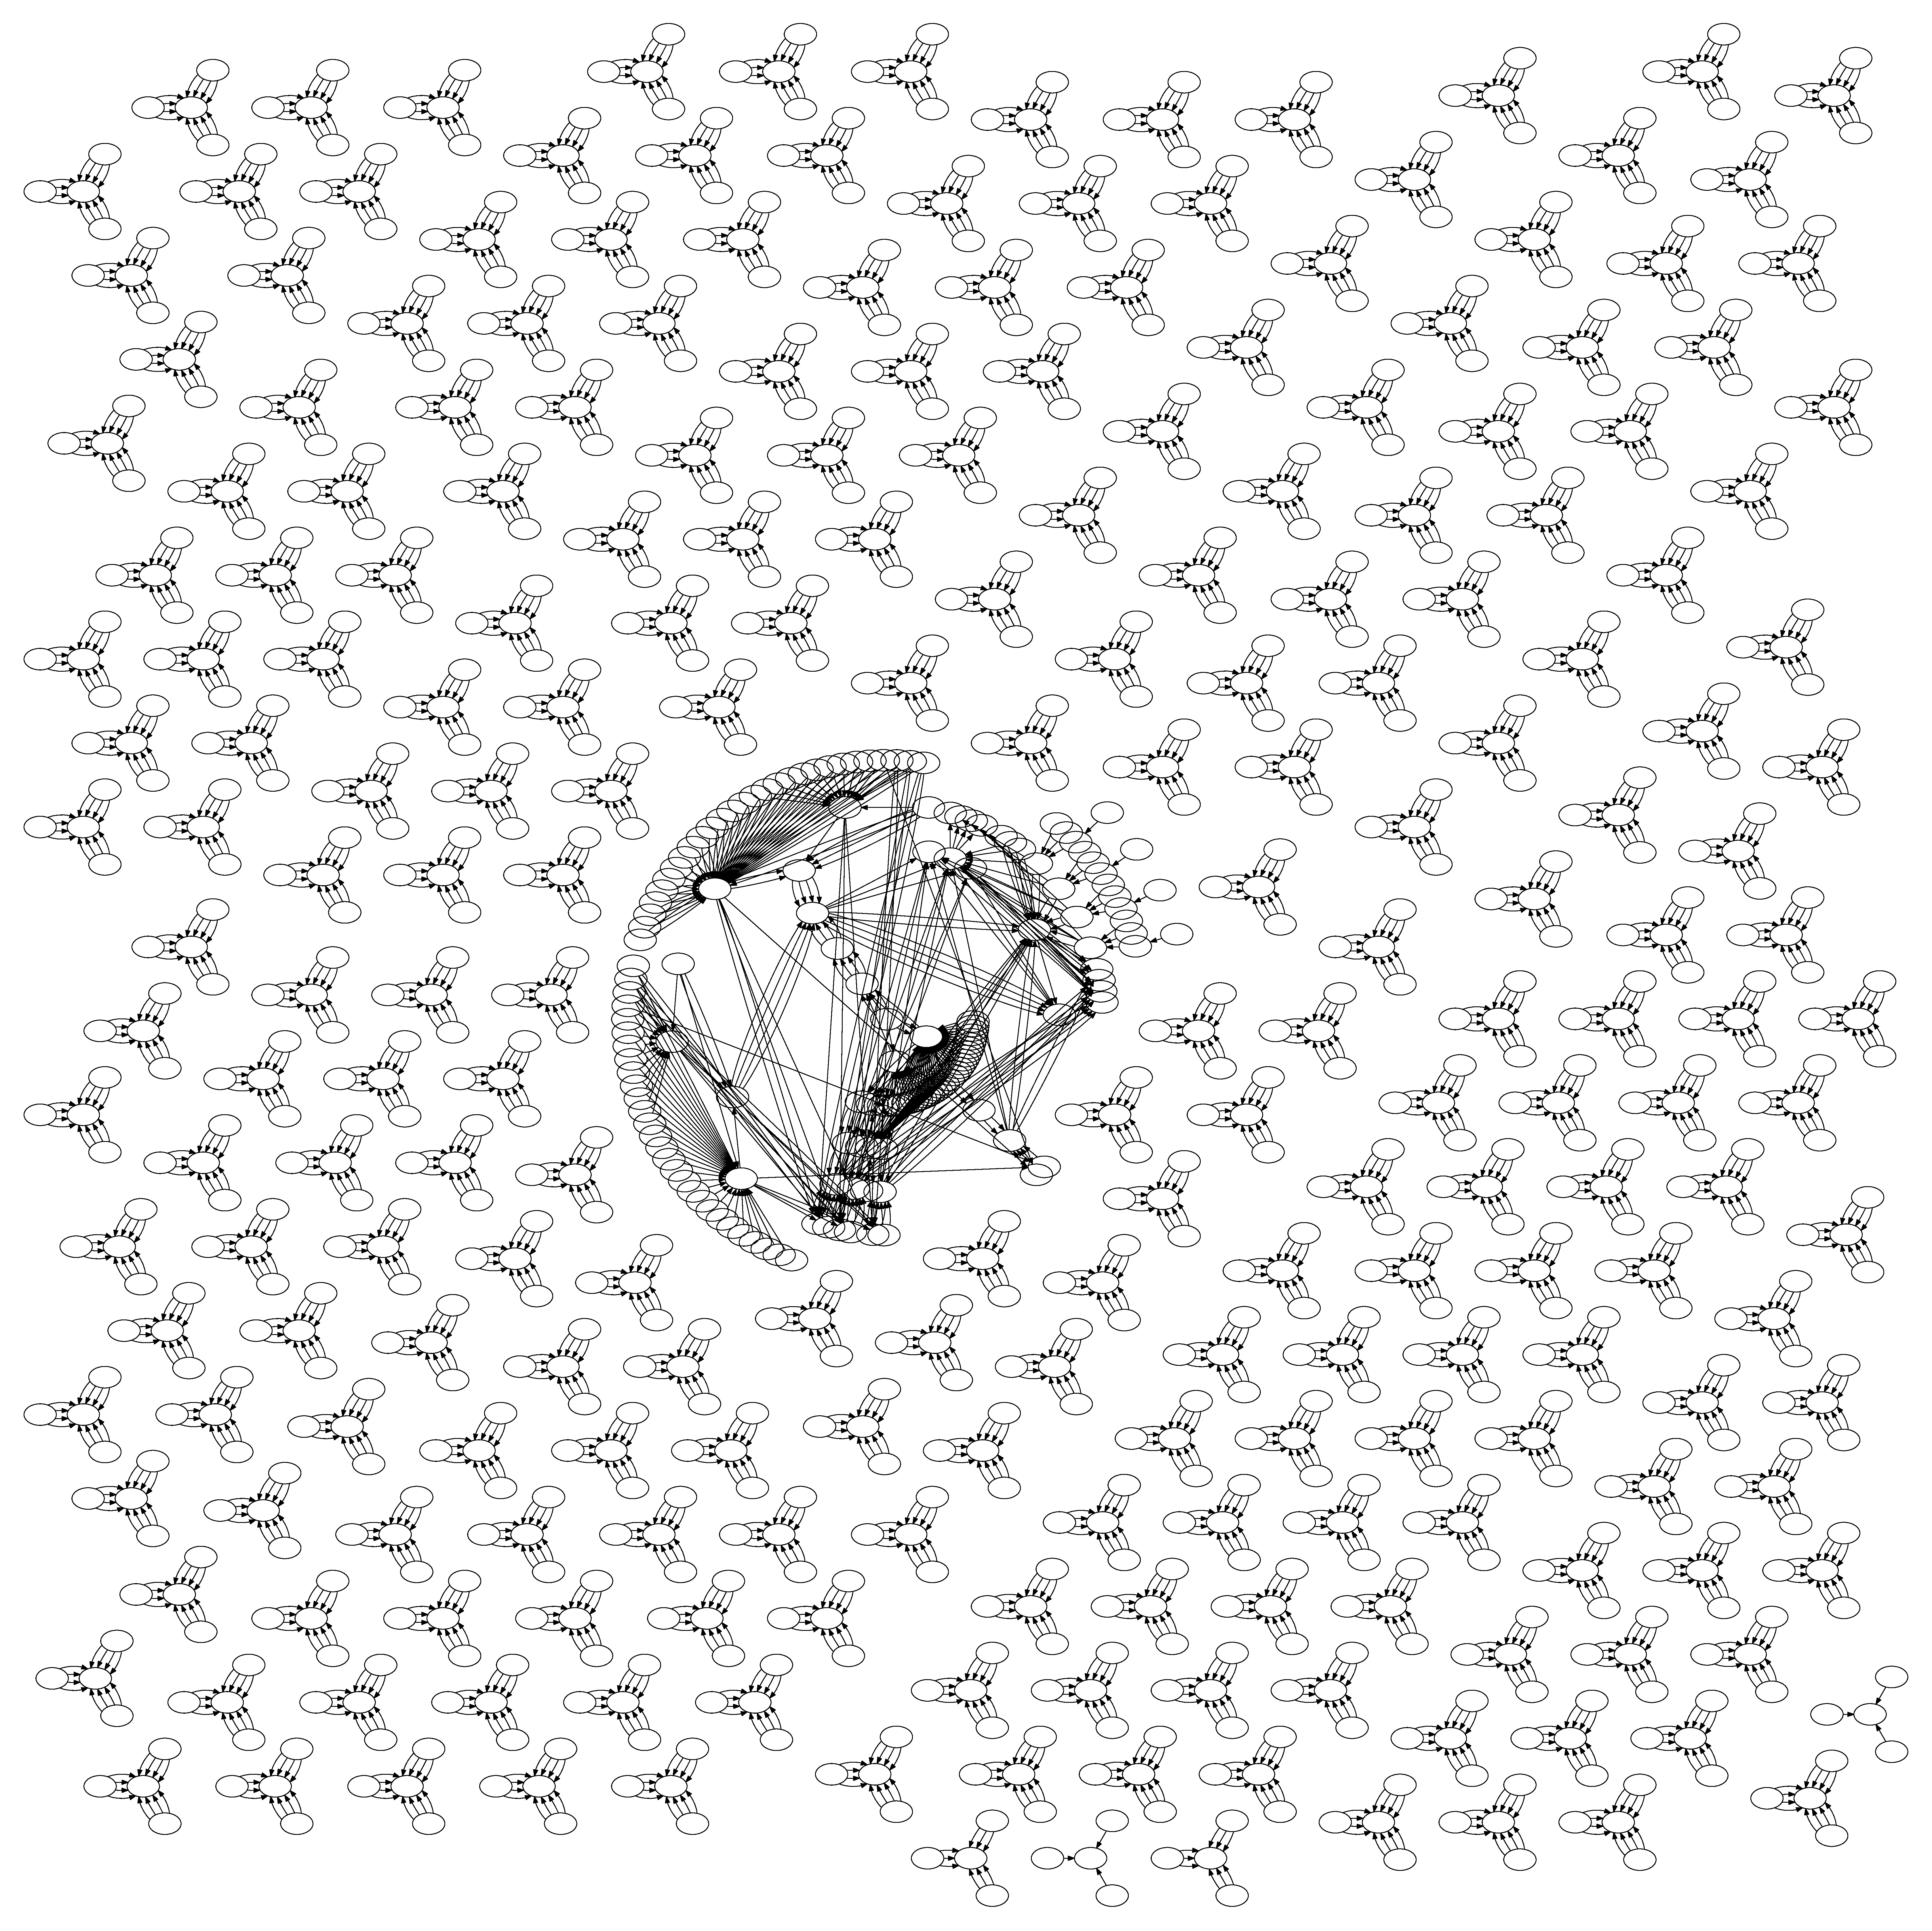
\includegraphics[width=7in]{intresults_tree}
  \caption{A dataflow graph for the \texttt{intresults} spreadsheet.  The highly-connected clique in the center causes the impact analysis to dominate \checkcell{}'s runtime. \label{fig:intresults_tree}}
\end{figure*}

\begin{figure*}[!t]
\centering
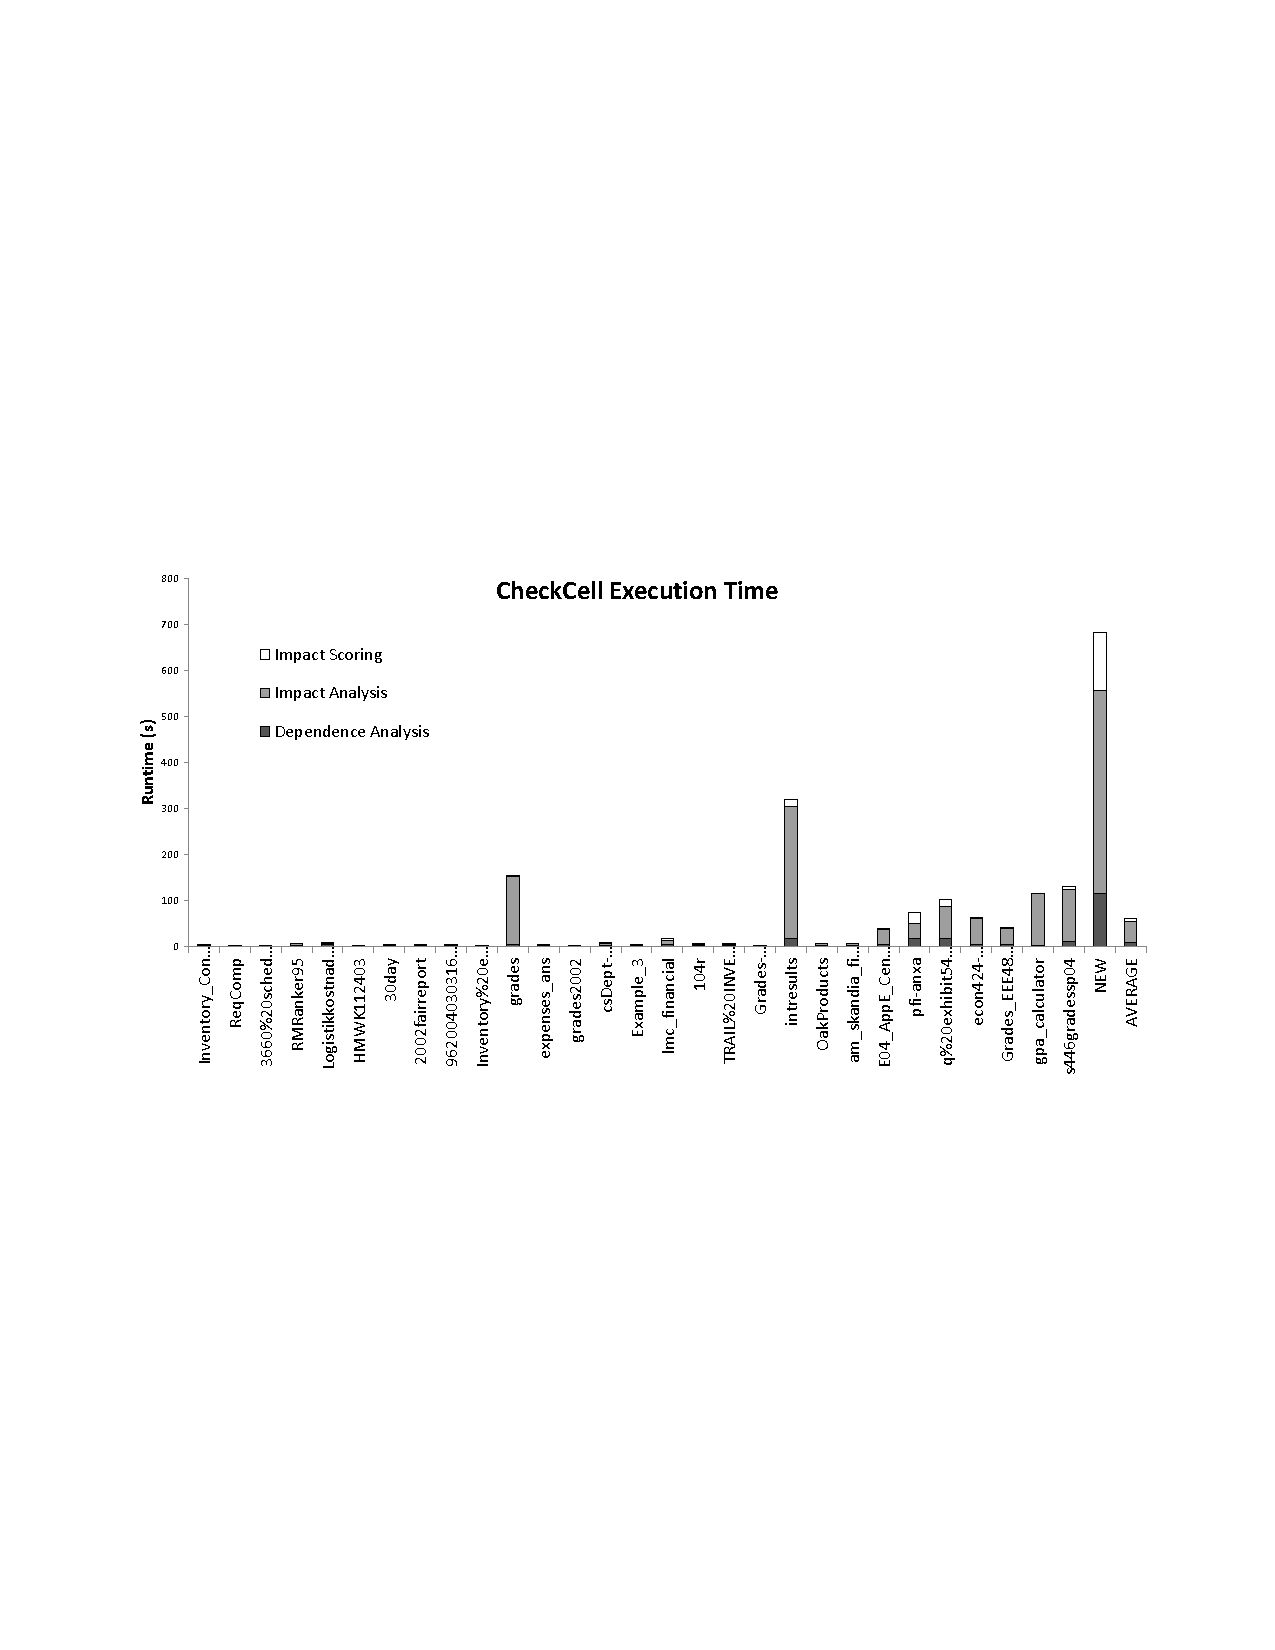
\includegraphics[width=5.5in]{execution_time_graph}
  \caption{\checkcell{} execution time. For most of the spreadsheets, \checkcell{} completes its analysis in under 9 seconds; for all but two, it completes in under three minutes (see Section~\ref{sec:execution_time}).\label{fig:execution_time_graph}}
\end{figure*}
 
Figure~\ref{fig:execution_time_graph} reports the performance of data
debugging across our spreadsheet suite, ordered by the weighted number
of cells. Table~\ref{tab:spreadsheet_characteristics} includes the full data.

For 19 of the 30 spreadsheets, \checkcell{} takes 9 seconds or less to
complete. Its runtime is less than three minutes for all but two of
the spreadsheets: \texttt{intresults} and \texttt{NEW}, which take 318
seconds and 683 seconds, respectively. The average runtime over all
spreadsheets is 61 seconds; without the two outliers, it is 29
seconds. As our analysis in Section~\ref{sec:asymptotic_analysis}
predicts, the cost of \checkcell{} is generally proportional to the
cost of the impact analysis, which is in turn dependent on the
weighted number of cells.

The spreadsheets that require the most execution time both have by far
the largest number of formulas (1,066 and 2,626), and the latter also
has the largest number of weighted cells (2,403). Their relatively
high execution time is attributable to the fact that cost of impact
analysis increases as the number of formulas increases, since the
Excel recalculation engine must do more work per item tested.

\paragraph{Summary:} For nearly every spreadsheet
 examined, \checkcell{}'s runtime is under three minutes; we believe
 this overhead is acceptable for an error detection tool.

% Info about the benchmarks.

% \subsection{Benchmarks}

%\subsection{Case Studies}

% \paragraph{9-Grades}

\subsection{Error Detection}
\label{sec:user_study}

While \checkcell{} can be used across the EUSES suite, looking for
errors in existing spreadsheets is problematic because we do not know
what the ground truth is. To evaluate \checkcell{}'s efficacy at
finding actual errors, we need errors and ground truth to compare it
against.

Rather than artificially inject errors, we designed an experiment that
allows us to observe real errors produced by people and use
\checkcell{} to find them. We collect human errors by hiring workers
to perform data entry tasks (entering known data) via Amazon's
Mechanical Turk, a popular crowdsourcing platform, and then check
their results with \checkcell{}.

Our ground truth data is drawn from \texttt{3q2000.xls}, a
spreadsheet from the EUSES repository that contains selected financial
information from Fannie Mae. We save the data as a comma-separated
value file (.csv). Mechanical Turk workers were paid 3 cents to
enter 10 of these numerical values at a time into a web form designed to look
like a spreadsheet, shown in Figure~\ref{fig:mturk_task}. To prevent
copying and pasting, we generate an image containing the
comma-separated values. Each worker had the opportunity to perform up
to seven different tasks.

In all, we collected 200 responses from 46 distinct users. Out of
these responses, 14 had omitted data and 52 contained errors, for an
overall error rate of 33\%. The errors can be classified into the following categories:

\begin{itemize}
\item \textbf{Sign omission}, where a negative sign was dropped
\item \textbf{Magnitude error}, any change in a value (usually a dropped or spurious digit) that results in an order of magnitude increase or decrease
\item \textbf{Digit transposition}, where at least two digits are transposed
\item \textbf{Typo}, any other typographical error (a mistyped digit)
\end{itemize}

We then inserted the erroneous data back into the spreadsheet one at a
time and ran \checkcell{} to see whether it found any of these
errors. Recall that by design, \checkcell{} reports data with an
unusual impact on any of the calculations. For this
spreadsheet, \checkcell{} always highlights the values in the top row
(the net interest income) because these values have a significant
impact on the spreadsheet; most of the income in this spreadsheet
comes from this row. We classify \checkcell{} as having correctly
found an error if it also highlights an erroneous cell.

For 13 of the 52 erroneous inputs (25\%), \checkcell{} correctly marks
the cell with the error, verifying our hypothesis that locating data
with unusual impact also finds errors. In all but two of these cases,
the error was a magnitude error; such errors are likelier to have an
unusual impact on a computation than all other errors, since they
change the input data dramatically. Even sign omission only causes a
factor of two change in a data element. Nonetheless, 20 of the errors
that \checkcell{} does not report also involve magnitude errors, but
those errors occur in data that do not contribute significantly to any
computation.


\begin{figure*}[!t]
\centering
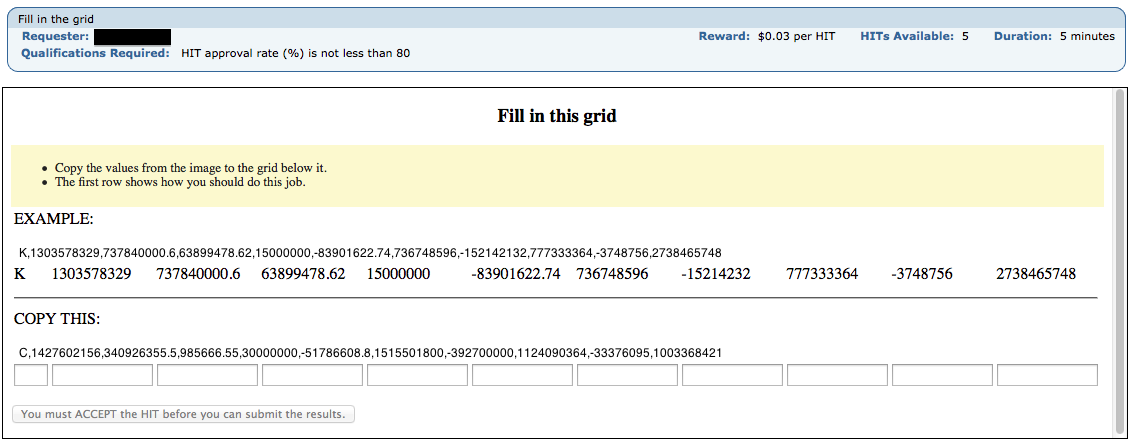
\includegraphics[width=5.5in]{images/mturk_fuzz_task}
  \caption{The page presented to Mechanical Turk workers to perform data entry tasks in order to collect actual human data entry errors (see Section~\ref{sec:user_study}).\label{fig:mturk_task}}
\end{figure*}


\begin{figure*}[!t]
\centering
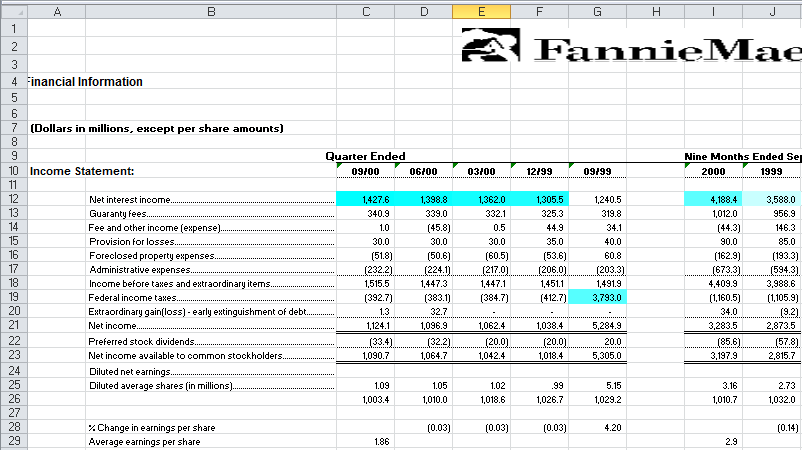
\includegraphics[width=5.5in]{images/fannie_mae_outlier}
  \caption{A screenshot of \checkcell{}'s results. In addition to the top row, which has a large impact on the final results, \checkcell{} highlights cell \texttt{G19}, a human data entry error.\label{fig:fannie_mae}}
\end{figure*}

Figure~\ref{fig:fannie_mae} presents a screenshot of \checkcell{}'s
results with one of these errors. In addition to the top
row, \checkcell{} indicates that cell \texttt{G19} has an unusual
impact; this is, in fact, the error. The correct value
for \texttt{G19} is \texttt{-379300000}, and the value entered by the
worker was \texttt{3793000000}: the worker made both a sign error and
an order of magnitude error (one too many 0's).

\paragraph{Summary:} By searching for data with unusual impacts on the spreadsheet, \checkcell{} is able to successfully find actual human data entry errors.




\subsection*{Proposed Work}
%\section{Proposed Work 1: Static Analysis}

%\todo{FIX ME}


\section{Medium-Scale Data Debugging: Relational Databases} % (fold)
\label{sec:bi_directional}

We propose to apply data debugging techniques to perform data cleaning
on relational data.  Cleaning tools attempt to purge datasets of
discrepancies before the data can be used, but many errors still go
undetected and get propagated further through queries and other
transformations. When errors are detected in transformation results,
it is critical to trace them back to their source and correct them to
prevent them from affecting other computations. Data debugging can
facilitate \emph{post factum} cleaning by identifying the input data
with the highest contributions to an incorrect result. We propose to
combine two methods of impact analysis in large-scale relational
datasets: forward and reverse analysis.

\subsection{Forward Analysis} % (fold)
\label{sub:forward_analysis}

The approach outlined in Section~\ref{sec:overview} relies on
re-calculating computations either exhaustively, or using random
sampling over a range of data. In a database setting, this approach
can be viewed as an extreme form of \emph{forward analysis}: an
analysis that starts with data and observes its effect on a
query. Previous forward analyses in database research include
\emph{hypothetical}, or \emph{what-if} queries
\cite{DBLP:conf/vldb/BalminPP00,DBLP:conf/icde/LakshmananRS08}: a
query result is computed based on a (single) hypothetical change to
the input data. Data debugging requires invoking multiple what-if
queries to find values with inordinately high impacts.

Forward analysis is powerful because it does not require any knowledge
of the inner workings of the computation, but for database systems,
directly adopting the data debugging approach outlined earlier would
be inefficient. Computing the transformation itself may be
computationally intensive, and calculating the exact impact of each
input tuple would require an exhaustive search over the input domain.

One way to reduce the cost of data debugging in databases is to peel
back the black box abstraction, as described in our proposed work for
spreadsheets.  The black box abstraction makes it particularly
suitable for user-defined functions (UDF). However, many computations
in the relational model rely on SQL transformations, which are simple
to analyze.

% Exploiting knowledge of the data transformations can
%improve performance, but requires lifting the black box assumption.

% In this setting, the black box model is too restrictive.


% Forward analysis is inefficient and does not scale to complex problems: computing the transformation itself may be computationally intensive, and calculating the exact impact of each input tuple requires an exhaustive search over the input domain. 
% Calculating impact over sets of input tuples makes the problem even harder, as it causes combinatorial explosion of the search space. 
%Lifting the black box assumption can often do much better. 
% We revisit the personal budget example discussed in Section~\ref{sec:overview}. If we know the function that computes cell \texttt{B12}, we can calculate the impact of a cell \texttt{B$_j$} as follows:
% \begin{align}\label{eqn:example_reverse}
% 	\sum_{i\neq j} I(\texttt{B}_j - \texttt{B}_i > \texttt{B}11-\texttt{C}11-150) = \sum_{i\neq j} I(\texttt{B}_j - \texttt{B}_i >3520.92)
% \end{align}
% where $I$ is an indicator function. Therefore, we can determine the impact of an input value without recomputing the function. SQL transformations are particularly amenable to such optimizations. 

Consider the following example SQL query, where the inner subquery
returns all departments that have a branch in Boston, and the outer
query computes the average salary of the employees that do not work in
any of those departments.

%The following nested SQL query returns the average salary of all employees who do not work for a department that has a branch in Boston.
\texttt{
\begin{tabbing}
		SELECT	\=avg(E.salary)\\
		FROM	\>Employees E\\
		WHERE	\>E.department NOT IN	(\=SELECT	\=distinct D.name\+\+\\
										FROM	\>Department D, Branches B\\
										WHERE	\>D.did = B.did AND B.location = `Boston')
\end{tabbing}}

\noindent
In this example, we do not need to recompute the nested subquery if
only the \texttt{Employees} table is modified during impact
analysis. SQL queries are particularly amenable to such optimizations.

% \comment{In a relational setting, impact analysis also needs to account for functional dependencies and other database-enforced constraints (e.g. foreign-key constraints). These would restrict the modifications that we can apply to the input. Is this interesting/important enough to mention here?}

% \comment{Possible argument against black box: ``weird'' functions like parity.}

% subsection forward_analysis (end)

\subsection{Reverse Analysis} % (fold)
\label{sub:reverse_analysis}
Forward impact analysis is not well-suited for certain errors that
result from data integration. To address these cases, we propose \emph{reverse analysis}. This technique analyzes transformations, such as SQL queries, and effectively inverts them to derive an input from a given output.

Data in databases often comes from multiple
sources, and is collected via multiple methods. In practice, databases are
often produced by merging other existing databases, and this process can
introduce redundancies and inconsistencies. Data integration errors are often identified by the violation of key constraints and other functional dependencies. Figure~\ref{fig:integrationExample} demonstrates a key-constraint violation after merging two relations. A database needs to satisfy several, often complex constraints, and the cleaning task may specify additional constraints or objectives.

\begin{figure}
	\small{\begin{tabular}{|l|l|l|l|l|l|l|l|}
		\multicolumn{5}{c}{Input tables} & \multicolumn{1}{l}{}& \multicolumn{2}{c}{Integration result}\\
		\multicolumn{5}{c}{$\overbrace{\rule{9.5cm}{0pt}}$} & \multicolumn{1}{l}{}& \multicolumn{2}{c}{$\overbrace{\rule{4.5cm}{0pt}}$}\\
		\multicolumn{2}{l}{Products (A)} & \multicolumn{1}{l}{} & \multicolumn{2}{l}{Products (B)} & \multicolumn{1}{l}{} & \multicolumn{2}{l}{All Products}\\
		\cline{1-2}\cline{4-5}\cline{7-8}
		\textbf{\underline{ItemNum}} & \textbf{product name} & \multicolumn{1}{l|}{} & \textbf{\underline{ItemNum}} & \textbf{product name} & \multicolumn{1}{l|}{} & \textbf{ItemNum} & \textbf{product name}\\
		\cline{1-2}\cline{4-5}\cline{7-8}
		5253B002 & Nikon D4 SLR & \multicolumn{1}{l|}{} & 5253B002 & Nikon D4 digital & \multicolumn{1}{l|}{} & 5253B002 & Nikon D4 SLR\\
		\cline{1-2}\cline{4-5}\cline{7-8}
		25482 & Canon EOS 1D X & \multicolumn{1}{l|}{} & 25482 & Canon 1DX EOS & \multicolumn{1}{l|}{} & 5253B002 & Nikon D4 digital\\
		\cline{1-2}\cline{4-5}\cline{7-8}
		\multicolumn{6}{l|}{} & 25482 & Canon EOS 1D X\\
		\cline{7-8}
		\multicolumn{6}{l|}{} & 25482 & Canon 1DX EOS\\
		\cline{7-8}
		
	\end{tabular}}
	\caption{ItemNum is a key (its value is unique) in the input tables, but the same is not true for the integration result. The integrated data needs to be cleaned to produce a valid data instance.}\label{fig:integrationExample}
\end{figure}

\begin{example}\label{ex:how-to}
A manufacturing company orders parts from multiple suppliers around
the world. To reduce its dependence from any single country, the
company makes sure that its inventory orders from each country do not
exceed 10\% of all orders. However, after merging with another
manufacturer, this condition is no longer satisfied. The company needs
to ``clean'' its inventory orders by reassigning some orders to
different suppliers. Ideally, it would like to achieve this with the
minimum number of changes.
\end{example}

Example~\ref{ex:how-to} presents a data cleaning scenario which is not
well suited for forward analysis. In the presence of complex
conditions, forward impact analysis has to exhaustively search all
possible scenarios.

In previous work, we have modeled these scenarios with \emph{how-to}
queries: ``how should the input change in order to achieve the desired
output?''~\cite{DBLP:journals/pvldb/MeliouGS11} How-to queries are an
example of reverse analysis. In contrast to forward analysis,
reverse analysis specifies the desired effect on the output, and
reverse engineers how the input should change. Reverse analysis has
more complex semantics and higher implementation complexity compared
to forward analysis due to the fact the inverse of a function is not
always a function. Given a desired output, there may be multiple input
values (or none at all) that produce it.  As opposed to forward
analysis, reverse analysis cannot handle black box computations, but
uses knowledge of the transformations to perform the evaluation
efficiently.

%To circumvent this difficulty in a general framework we will use SAT and Mixed Integer Programming (MIP) solvers as general purpose tools in reverse analysis. 

% We propose to augment data debugging with \emph{reverse impact analysis}. In contrast to forward analysis (``how would the output change for a given change in the input''), reverse analysis answers the question ``how should the input change in order to achieve the desired output?'' 

The Tiresias system~\cite{DBLP:conf/sigmod/MeliouS12,
  DBLP:conf/sigmod/MeliouSS12}, developed by PI Meliou, can
efficiently evaluate how-to queries, and is used for complex cleaning
tasks such as the one in Example~\ref{ex:how-to}. How-to queries are
constraint optimization problems defined over relational data, but
they cannot be expressed in standard SQL. Tiresias allows users to
issue how-to queries through a declarative language based on
Datalog~\cite{DBLP:journals/tkde/CeriGT89}, and the queries are
evaluated using mixed integer programming solvers.

\paragraph{Calculating impact.} % (fold)
\label{par:calculating_impact}

Tiresias does not quantify the impact of input data, but rather
produces an instance of the input that satisfies all cleaning
constraints. In prior work, PI Meliou introduced a theory of causality
for relational databases~\cite{DBLP:journals/debu/MeliouGHKMS10},
which can model impact under the reverse analysis model. It is
possible to characterize the family of conjunctive queries for which
\emph{responsibility}---the contribution of an input to a result---can
be computed in polynomial
time~\cite{DBLP:journals/pvldb/MeliouGMS11}. Tiresias uses SAT solvers
to compute responsibility efficiently for NP-hard
cases~\cite{DBLP:conf/sigmod/MeliouGNS11}.

% paragraph calculating_impact (end)

% Halpern and
%Pearl~\cite{HalpernPearl:Cause2005} and Chockler and
%Halpern~\cite{DBLP:journals/jair/ChocklerH04} gave mathematical
%definitions of causality and its related notion of degree of
%responsibility. Responsibility quantifies  

% subsection reverse_analysis (end)


%--------------------------------------------------------------------------

\subsection{Proposed Work} % (fold)
\label{sub:research_plan}

Complex transformations contain both glass box and black box
components. We propose to develop a \textbf{bi-directional data
  cleaning} framework that combines both forward and reverse
analysis. This framework can flexibly adapt to different types of
computations. We will investigate the following research questions:

\paragraph{Static analysis of SQL queries.} % (fold)
\label{par:static_analysis_of_sql_queries}
SQL queries are the primary type of computation in relational databases. We will investigate techniques to break down queries into \emph{active} and \emph{inactive} components: active components are the parts of the query that need to be recomputed during forward analysis, whereas inactive are components that compute intermediate results that don't change and thus can be precomputed. This is a hard problem as it relates to the problem of query containment, which is undecidable~\cite{DBLP:conf/pods/CalvaneseGL98}.
% paragraph static_analysis_of_sql_queries (end)

\paragraph{Cleaning optimizations.} % (fold)
\label{par:cleaning_optimizations}
In complex transformations, it is not clear how forward and reverse analysis
should be combined. We will use computational patterns to design a cleaning
optimizer, modeled after traditional relational query optimizers. Given a
cleaning task, the optimizer should select how to subdivide the task into the
forward and reverse components, and in which order the tasks should be
performed.
% paragraph cleaning_optimizations (end)

\paragraph{Interactive cleaning.} % (fold)
\label{par:interactive_cleaning}
Cleaning tasks are often based on complex constraints, and have many possible
solutions. It can be a daunting undertaking for a user to assess these
solutions, or even define the cleaning task itself. We will design an
interactive interface to allow users to easily identify possible problems, and
we will investigate techniques to refine solutions based on user feedback.
% paragraph interactive_cleaning (end)



% subsection research_plan (end)



% section bi_directional (end)


\section{Large-Scale Data Debugging: MapReduce}
\label{sec:mapreduce}

Large-scale data-parallel computation is increasingly important.
Technologies such as MapReduce provide useful functional programming
constructs for parallelizing compute-intensive jobs.  However,
debugging data-parallel programs remains difficult, particularly with
regard to errors in giga-, tera-, and peta-scale inputs. 

While it may seem at first glance that ``big data'' problems should be
inherently robust to errors in their input, this is not necessarily
the case. Regardless of the robustness of the computation being
performed, the computation is likely to be wrong whenever data sources
(e.g., sensor data or data files) have been corrupted, or when data is
systematically biased because of miscalibration. Even small errors can
have large effects in the face of threshold functions or certain
mathematical computations. For example, the presence of a single zero
value can result in catastrophic cancellation; the same is true for
order-of-magnitude errors.

\subsection{Proposed Work}

Correcting individual errors in large-scale datasets is likely
to be infeasible, so we propose to use data debugging techniques to
automatically make large-scale computations more robust. The key idea
is to run data debugging alongside MapReduce jobs and compensate for
errors automatically by performing what we term \emph{input
  trimming}. With input trimming, MapReduce jobs produce the results
both for the original dataset and for a version of the dataset with
unusually-impactful data elements removed. The user can then compare
the results of both computations. When both match, there is no
problem. When they diverge, data debugging can report summaries of the
values and their data sources to point programmers to possible
problems with input data.


\begin{figure*}[t]
	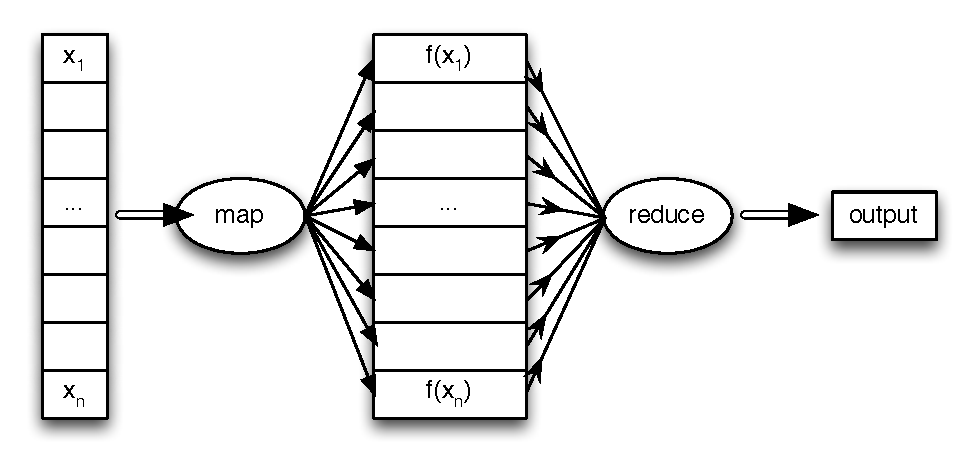
\includegraphics[width=2.5in]{images/mapreduce}
  % \hspace{30px}
  \hfill
	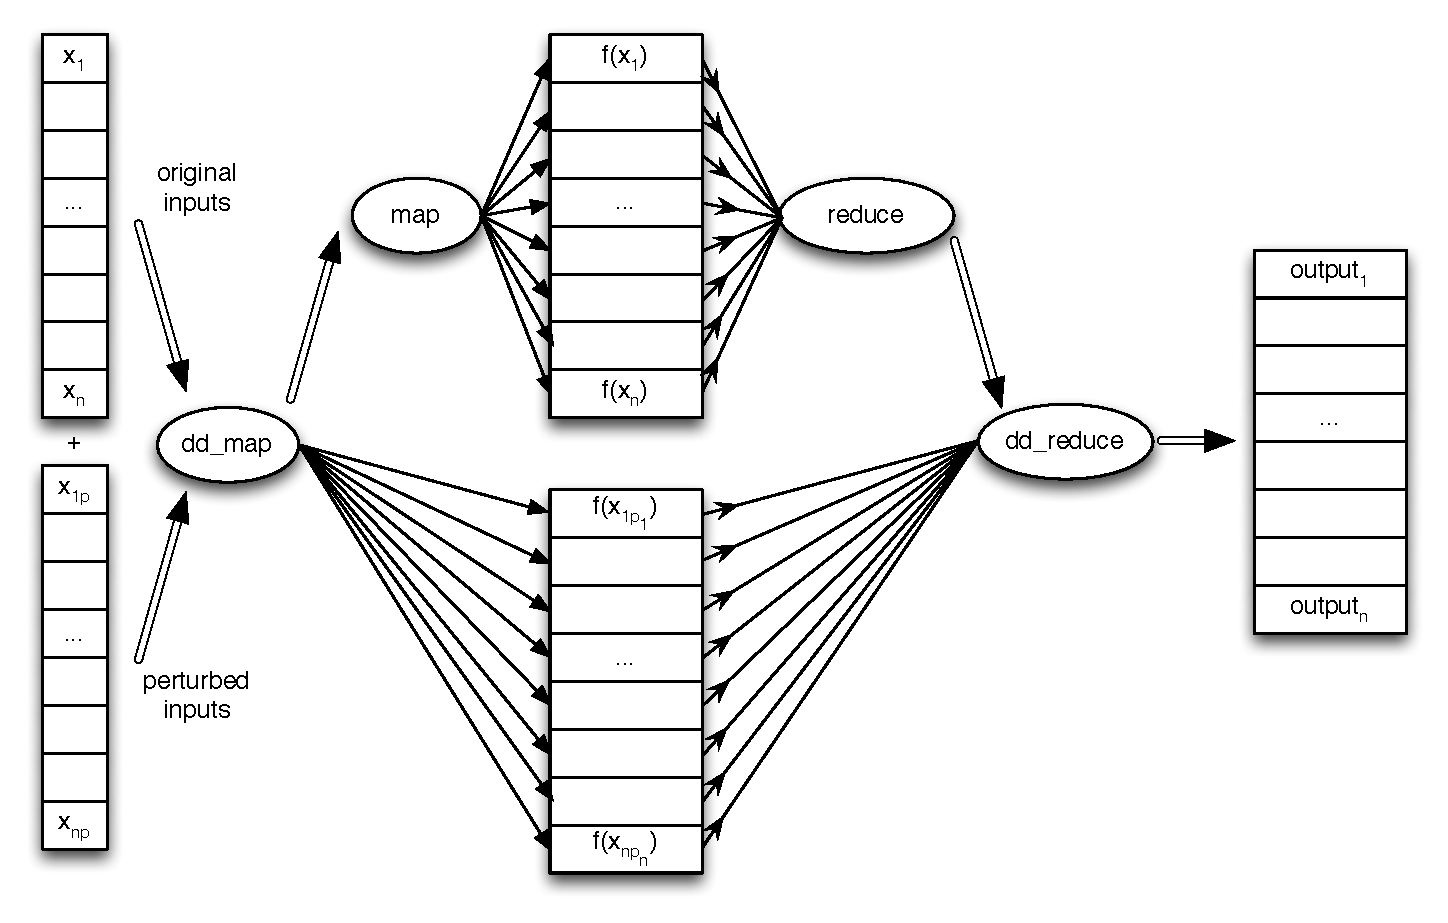
\includegraphics[width=3.25in]{images/mapreduce_dd}
	\caption{
		On the left, a typical MapReduce job.  On the right, a data debug-augmented MapReduce job.  Each additional output is a version of the computation with the unusually impactful values automatically excluded.\label{fig:mapreduce_pipeline}
	}
\end{figure*}

\paragraph{MapReduce-Based Frameworks.}
While MapReduce and Hadoop jobs are low-level programming idioms,
frameworks like FlumeJava (and by extension, its Hadoop-based clone, Crunch)
allow multi-stage MapReduce programs to be represented by higher-level
programming constructs~\cite{pldi:flumejava}.  These constructs allow
the runtime to determine a program dependency graph.  This
higher-level representation gives the runtime global information that
facilitates automatic performance-enhancing program transformations,
such as reordering of functions in the program call graph to increase
parallelism.

We observe that data-parallel programs constructed in this fashion
share many of the same properties that make data debugging a useful
technique in spreadsheets.  The input to the mapper stage of a
MapReduce problem is a large, homogeneous vector amenable to the same
kind of input perturbation that \checkcell{} employs.  A key property
of the computation kernel in a MapReduce job is that code is
shared-nothing and re-entrant. Therefore, data debugging (which often
needs to recompute certain portions of the call graph) can be inserted
into a portion of a MapReduce job without affecting the semantics of
the original program.

\paragraph{Data Debugging for Robustness.}
As with \checkcell{}, data debugging functions can transparently
augment a FlumeJava program.  The tradeoff is a small performance
penalty for the additional robustness that data debugging provides. Data
debugging techniques can be piggybacked on a high-level representation
so that impact analysis can take advantage of underutilized
parallelism to minimize the performance impact of our technique.

To be feasible, large-scale data debugging requires at least two kinds
of program transformations.  First, a data debugging-enhanced library
like FlumeJava would augment the map stage with perturbed input values
to be computed in parallel, and the reducer function would be
augmented with the impact computation.  Our implementation of
\checkcell{} relies on Microsoft Excel's ability to recognize when
partial recomputation of the dependency graph is possible for
efficiency purposes. A data debugging-enhanced FlumeJava runtime would
need to recognize when an impact calculation may be performed for
only a subset of the program dependency graph, and when the dependency
analysis itself contains overlapping subproblems whose solutions
should be shared to improve performance.

Once impact scores are known for a set of MapReduce program inputs,
the data debugging runtime can be instructed to re-run the computation
with the unusually impactful inputs either removed or replaced with
user-specfied values.  The degree of unusualness, in terms of standard
deviations from the norm, may be used to control the degree of
input trimming performed on the MapReduce input vector.  Again,
a high-level representation of the program graph allows this
recomputation to be performed for the minimum cost possible.


%\input{jsbackground}
%\input{static-lang}
%\input{dynamic-lang}
%\input{opt}
%\input{codegen}
%\input{system-support}

% The formula here is: discuss related work in one facet; end with a contrast with the current work.

\paragraph{Data Cleaning.}
Most past work on locating or removing errors in data has focused
on \emph{data cleaning} (also known as \emph{data scrubbing}
and \emph{cleansing}) in database
systems~\cite{DBLP:journals/debu/RahmD00,han2006data}. Standard
approaches include statistical outlier analysis for removing noisy
data~\cite{1583581}, interpolation to fill in missing data (e.g., with
averages), and using cross-correlation with other tables to correct or
locate errors~\cite{Hernandez:1995:MPL:223784.223807}.

% Also: noise removal.

% Section~\ref{FIXME} shows that statistical outlier analysis often produces unacceptably large numbers of false positives. 

% SURVEY! http://www.dbis.informatik.hu-berlin.de/dbisold/research/bioinformatics/papers/data_cleansing.html

A number of approaches have been developed that allow data cleaning to
be expressed programmatically or applied interactively. Programmatic
approaches include AJAX, which expresses a data cleaning program as a
DAG of transformations from input to
output~\cite{Galhardas:2000:AED:342009.336568}. Data Auditor applies
rules and target relations entered by a
programmer~\cite{Golab:2010:DAE:1920841.1921060}. A similar
domain-specific approach has been employed for data streams to smooth
data temporally and isolate it spatially~\cite{1617508}. Potter's
Wheel, by Raman and Hellerstein, is an interactive tool that lets
users visualize and apply data cleansing
transformations~\cite{Raman:2001:PWI:645927.672045}. 
Luebbers et al. describe an interactive data mining approach based on
machine learning that builds decision trees from databases. It marks
deviations from derived logical rules (e.g., ``$\mbox{BRV} =
404 \Rightarrow \mbox{GBM} = 901$'') as errors to be examined by a
data quality engineer~\cite{Luebbers:2003:SDD:1315451.1315499}.

Unlike these approaches, data debugging operates entirely
automatically (without the need for programmer-supplied rules or
latent logical relations in data) by measuring the interaction of data
with the programs that operate on them.
 

\paragraph{Spreadsheet Errors.}
Spreadsheets have been one of the most prominent computer applications
since their creation in 1979.
 The most widely used spreadsheet application today is Microsoft
Excel. Excel includes rudimentary error detection including errors in
formula entry like division by zero, a reference to a non-existient
formula or cell, invalid numerical arguments, or accidental mixing of
text and numbers.
% http://office.microsoft.com/en-us/excel-help/find-and-correct-errors-in-formulas-HP010066255.aspx
Excel also checks for inconsistency with adjacent formulas and other
structural errors, which it highlights with a ``squiggly'' underline. In addition, Excel provides a formula auditor, which lets spreadsheet view dependencies flowing into and out of a particular formula.
% http://office.microsoft.com/en-us/excel-help/use-error-checking-to-correct-common-errors-in-formulas-HA010342331.aspx

Past work on detecting errors in spreadsheets has focused on inferring
units and relationships (has-a, is-a) from information like layout and
headers~\cite{DBLP:conf/kbse/AhmadAGK03}. XeLda checks if formulas
process values with incorrect units or if derived units clash with
unit annotations~\cite{Antoniu:2004:VUC:998675.999448}.  More type
system stuff:~\cite{Erwig:2005:AGM:1062455.1062494}. Using labels and
structural clues (especially unit-of-measurement
errors)~\cite{Chambers:2010:RSL:1860134.1860346}. There also has been
considerable work on testing tools for
spreadsheets~\cite{fisher2006scaling,rothermel1998you,rothermel2001methodology,Carver:2006:EET:1159733.1159775}). Much
of this work is complementary and orthogonal to \checkcell{}, which
works with standard, unannotated spreadsheets and focuses on unusual
interactions of data with formulas.


% What is Jaffry et al\. ~\cite{DBLP:journals/corr/abs-0803-1748}?

\paragraph{Outlier Analysis}

Techniques to remove outliers (unusual data) date to the earliest days
of statistics, when they were developed to make nautical measurements
more robust. Widely-used approaches include Peirce's criterion,
Chauvenet's criterion, and Grubb's test for outliers~\cite{barnett1994outliers}. All
of these techniques require that data belong to a known distribution,
primarily the normal (Gaussian). Unfortunately, input data does not
always fit any statistical distribution. Even when outlier detection is
possible, identifying them leads to false positives when they do not
materially contribute to the result of a computation.
\checkcell{} leverages the
fact that its statistical sampling approach forces observed effects to
follow a Gaussian distribution (as Section~\ref{sec:FIXME} explains),
allowing it to use the Peirce outlier test to determine whether a
particular value has an unusual impact on a computation.


\section{Broader Impact, Education, and Outreach}
\label{sec:impact}

\paragraph{Broader Impact.} 
FIX ME.

We will add to the national computing infrastructure by implementing
and making available all of the component
systems we build as part of this project.  These tools will add to the national research and industry
software infrastructure. Our prior tools are in wide use in industry
and academia, and we expect these will be also.

\paragraph{Education.}
We plan to integrate the research developed here into both
undergraduate and graduate classes. FIX ME.

\paragraph{Outreach.}
Improving participation in computer science from underrepresented groups
requires outreach at multiple levels; the PIs have a strong track record
of this work at both the undergraduate and graduate levels.

PI Berger has supervised undergraduate research and
mentored women and minority undergraduates. PI Berger has recruited undergraduates from
across the neighboring Five College consortium (which includes Amherst
and Hampshire Colleges, and two female-only undergraduate institutions,
Smith and Mt. Holyoke Colleges). FIX ME Alexandra stuff.

% PI Berger participated in a discipline
% CRA-W workshop for under-represented minorities in 2008.
 
\section{Results of Prior NSF Support}
\label{sec:prior}

\paragraph{Emery D. Berger} is a PI of three active NSF grants.

% Thus far, 8 graduate students have been funded in
% full or in part by these grants; one graduated with a PhD in 2006, and
% one in 2009.

% EAGER

Professor Berger is a PI in a collaborative project with Professor
Daniel Jim\'enez (Texas A\&M University): {\em SHF: Large:
Collaborative Research: Reliable Performance for Modern Systems} (NSF
CCF-1012195, \$550,000, August 2010-July 2013). This project aims to
deliver reliable performance on modern computer systems. By
introducing randomness into the way a computer runs programs, a
reliably performant system will significantly reduce the probability
that any small change will have a large impact on performance.  It has
thus far produced two publications by PI Berger, to appear at ASPLOS
and in ACM TECS ~\cite{proartis2013,stabilizer:asplos13}, and one
major software release: \textsc{Stabilizer}, a compiler and runtime
system that enables statistically sound performance evaluation.

Professor Berger is sole PI of {\em Programming the Crowd} (NSF
CCF-1144520, \$300,002, August 2012-December 2013). This project
introduces crowdprogramming, an approach that fully integrates human
and digital computation. In crowdprogramming, humans are modeled as
function calls in a standard programming language. This approach lets
programmers focus on programming logic, while the crowdprogramming
runtime system manages the critical tradeoffs between cost, time, and
data quality. We have released a crowdprogramming system
called \textsc{AutoMan} and reported on it at
OOPSLA~\cite{Barowy:2012:API:2384616.2384663}.

Professor Berger is a PI in a collaborative project with Professor
Michael Hicks (University of Maryland) and Professor Kathryn McKinley
(UT-Austin): {\em PASS: Perpetually Available Software Systems} (NSF
CCF-0910883, \$639,420, August 2009-July 2013). This project proposes
a transformative paradigm shift to ``perpetually available software
systems'' (PASS) that will make software more available and robust by
directly addressing errors in deployed software. Thus far, this
project has led to two publications by PI Berger at OOPSLA and
SOSP~\cite{Liu:2011:DED:2043556.2043587,Liu:2011:SPD:2048066.2048070},
and two major software releases: \textsc{Dthreads}, a deterministic
replacement for \texttt{pthreads}, and \textsc{Sheriff}, a system that finds or eliminates false sharing.

PI Berger has been supported by three previous NSF grants:

The first of these grants is
\emph{CAREER: Cooperative System Support for Robust High Performance}
(NSF CAREER CNS-0347339, \$477,000, June 2004-2009). The purpose of this project is to attack the growing
latency between main memory and disk with adaptive algorithms that
leverage cooperation between the compiler, runtime systems, and
operating system. It has thus far produced eight papers that have
appeared at PLDI, OSDI (2), OOPSLA, ISMM, MSP, and USENIX~\cite{feng05,hert05,hert05a,yang04,1267316,transparent2006usenix,flux06usenix,DBLP:conf/osdi/YangLBKM08}.

PI Berger was the sole PI of \emph{Probabilistically Correct
  Execution: Hardening Applications Against Error and Attack} (NSF
  CNS-0615211, \$300,000, September 2006-2009, no cost extension).
  Probabilistically correct execution is an approach that allows
  programs to execute correctly with high probability in the face of
  errors or attack, and functions by both \emph{randomizing} the
  runtime system and \emph{replicating} differently-randomized
  executables. This combination transforms unreliable software
  components into a quantifiably more reliable system. This grant has
  thus far produced four papers, two at PLDI, one at ASPLOS, and one
  at
  OOPSLA~\cite{1134000,1250736,1346296,DBLP:conf/oopsla/BergerYLN09}. One
  result of this work is DieHard, a freely-available system that
  increases the security and resilience to memory errors of
  C/C++-based applications; DieHard has been downloaded over 20,000
  times since its release, and directly inspired the Fault-Tolerant
  Heap included in Windows since version 7. Another product of this
  research, the DieHarder secure heap, an inspiration for the security
  hardening features incorporated into Windows 8.

PI Berger was also a co-PI of \emph{MRI: Cluster Acquisition for
Computational Research into Large Scale Data Rich Problems} (NSF
CNS-0619337, \$350,000, 9/1/2006--9/1/2008).



FIX ME add Alexandra's stuff.


\section{Summary}

\todo{Timeline}

We propose data debugging, an approach aimed at
finding potential data errors by locating and ranking data items based on their
overall impact on a computation. Intuitively, errors that have no
impact do not pose a problem, while values that have an unusual impact
on the overall computation are either very important or incorrect.
We present a prototype of the first data debugging
tool, \checkcell{}, which operates on spreadsheets. We evaluate
\checkcell{}'s performance analytically and empirically, showing that
it is reasonably efficient and effective at helping to find data
errors. \emph{FIX ME.}



}

\clearpage
{\singlespace \small
\bibliographystyle{abbrv}
\bibliography{ref,berger/emery,meliou,provenance}
}

%\clearpage
%\input{collaboration}
%\section{Research Schedule} % (fold)
\label{sec:research_schedule}

\paragraph{Year 1.} % (fold)
\label{par:year_1}
During year 1, we will focus on the static analysis of spreadsheet functions, and SQL queries. We will study different functions, patterns, and query types. We will start experimenting both with synthetic and real-world data early, to assess the performance gains of static analysis.  At the end of year 1, we will start to evaluate the performance trade-off between alternative strategies.
% paragraph year_1 (end)

\paragraph{Year 2.} % (fold)
\label{par:year_2}
During year 2, we will maintain our focus on small and medium scale data debugging. We will start to study optimization techniques based on static analysis. We will design and implement an optimizer for impact analysis in relational data, modeled after traditional database optimizers. Our design will be based on complexity results, and pattern-based heuristics.
As part of this work, we need to investigate query rewrites that may lead to more efficient impact calculations.
% paragraph year_2 (end)

\paragraph{Year 3.} % (fold)
\label{par:year_3}
During year 3, the PIs will focus their efforts on augmenting MapReduce pipelines with impact monitoring tools. \comment{add stuff here}
% paragraph year_3 (end)

% section research_schedule (end)

\end{document}
